\chapter{Comparación de una película continua y de una monocapa de nanopartículas como biosensores}
% top level followed by section, subsection

\label{section:A1}

En la sección \ref{section:sensLambda} se comparó la sensibilidad del supuesto modo plasmónico colectivo para una monoaapa de nanopartículas (NPs) de oro con radio un radio $a$ y una fracción de cubierta $\Theta$, predico por el modelo de esparcimiento coherente (Coherent Scattering Model, CSM) con las de los arreglos nanoestructurados propuestos en la literatura consultada \cite{danilov2018ultra,svedendahl2009refractometric}. En esta sección se calcula  la longitud de penetración $\xi$ y la figura de mérito de bulto $\textit{FoM}_B$ para una monocapa desordenada de NPs  de oro y de plata y se compara con la $\xi$ y la $\textit{FoM}_B$ de un sensor comercial, basado en los plasmones-polaritones de superficie (Surface Plasmon Polaritons, SPPs), para una película de oro y una de plata. En la Fig. \ref{fig:SPPCSM} se muestran los cálculos de la reflectancia en configuración ATR para una película de oro y una de plata ---donde se observa el SPP resaltado por la línea discontinua blanca---, ambas de grosor $d=50$ nm, y para una monocapa de NPs esféricas de oro (con $a=30$ nm y $\Theta=0.125$) y una de NPs de plata (con $a=40$ nm y $\Theta=0.1$) ---resaltando al supuesto modo  plasmónico colectivo con los puntos amarillos---; se consideró para todos los cálculos un sustrato con índice de refracción $n_s=1.5$ y una matriz de agua con $n_m=1.33$.

\begin{figure}[h!]\centering
\begin{tikzpicture}[scale=1]
\node[inner sep=0pt] (graf) at (.05,0){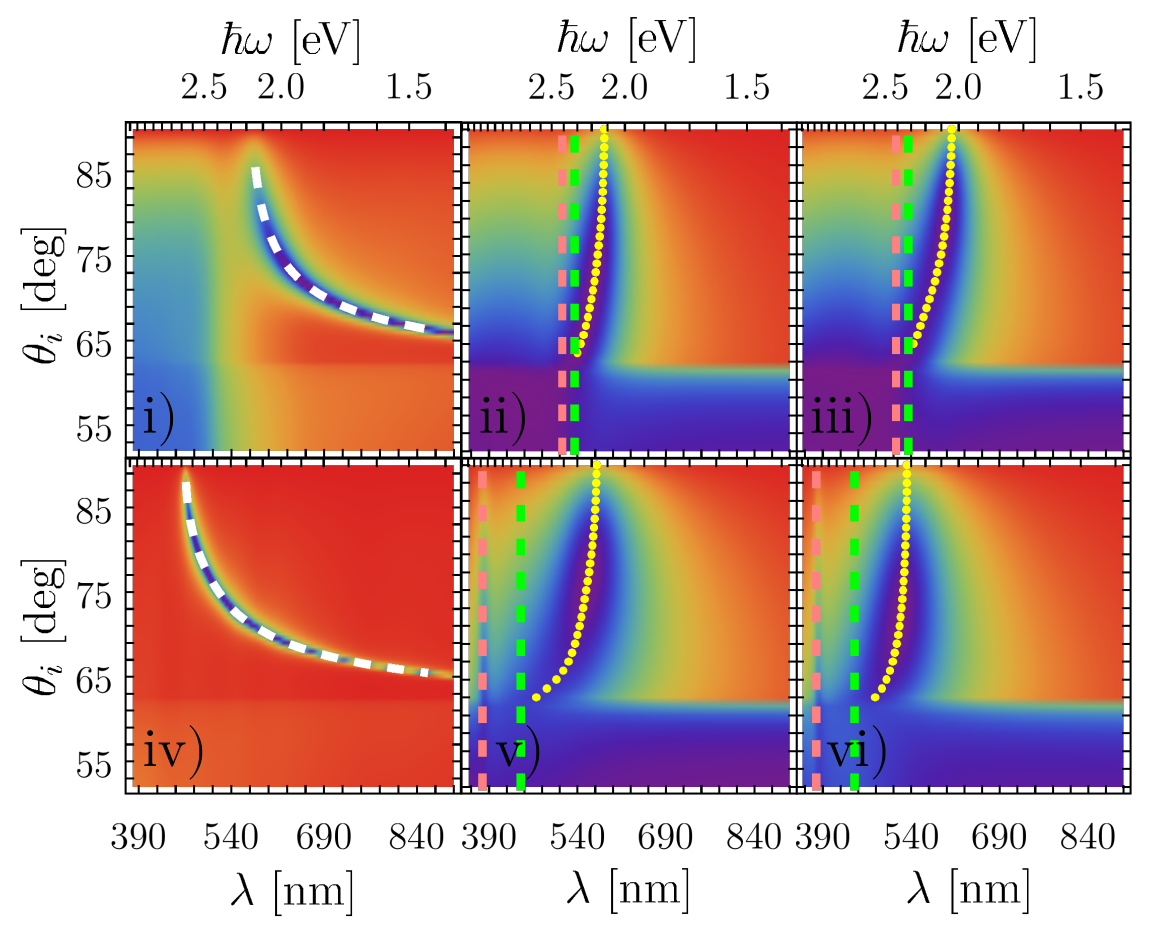
\includegraphics[scale=1]{2-Resultados/figs/11-SPPCSM/3-2D_Grid.png}};
\node[right, inner sep=0pt] (legend) at (4.4,.15) {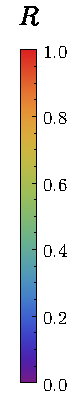
\includegraphics[scale=1, trim={00 -15 00 00}, clip]{2-Resultados/figs/0-RBar_v}};

\def\x{8}
\def\dy{.5}
	\node at(\x,3-\dy){\small i) SPP: Au, $d=50$ nm};
	\node at(\x,2.5-\dy){\small ii) CSM \emph{p}-Pol.:  NPs Au,};
	\node at(\x,2.-\dy){\small \;\;\; $a=30$ nm, $\Theta=0.125$};	
	\node at(\x,1.5-\dy){\small iii) CSM \emph{s}-Pol.:  NPs Au,};	
	\node at(\x,1.-\dy){\small \;\;\;   $a=30$ nm, $\Theta=0.125$};	
			

	\node at(\x,-1+\dy){\small iv) SPP: Ag, $d=50$ nm};
	\node at(\x,-1.5+\dy){\small v) CSM \emph{p}-Pol.: NPs Ag,};
	\node at(\x,-2+\dy){\small \;\;\;	 $a=40$ nm, $\Theta=0.1$};	
	\node at(\x,-2.5+\dy){\small vi) CSM \emph{s}-Pol.: NPs Ag,};
	\node at(\x,-3+\dy){\small \;\;\;  $a=40$ nm, $\Theta=0.1$};			

\def\xR{4.2}
\def\yR{2.5}	
	\node at(\xR,\yR){$R_s $};
	\node at(\xR,\yR-2.8){$R_s $};
	
	\node at(\xR-2.8,\yR){$R_p$};
	\node at(\xR-2.8,\yR-2.8){$R_p$};
	
	\node at(\xR-2*2.8,\yR){$R_p$};
	\node at(\xR-2*2.8,\yR-2.8){$R_p$};			
\end{tikzpicture}\vspace*{-.7em}
\caption{Gráficas de reflectancia $R$ en configuración ATR, considerando un sustrato con $n_s=1.5$ y una matriz con $n_m=1.33$, como función del ángulo de incidencia $\theta_i$ y de la longitud de onda $\lambda$ (escala inferior) así como de la energía en unidades de $\hbar\omega$ (escala superior), para una película delgada de $50$ nm de grosor (columna izquierda), y una monocapa de NPs esféricas iluminada por una onda plana en polarización \emph{p} (columna central) y en polarización \emph{s} (columna derecha); los paneles superiores corresponden a una película y NPs de oro con $a=30$ nm y $\Theta=0.125$, mientras que para los inferiores corresponden a una película y NPs de plata de con $a=40$ nm y $\Theta=0.1$.  Las líneas punteadas blancas (columna izquierda) corresponde a los mínimos en la reflectancia debido a la excitación del SPP y los puntos amarillos (columna central y columna derecha) corresponden a los mínimos en $R$ del supuesto modo plasmónico colectivo predicho por el CSM. Las líneas verticales punteadas verdes corresponden a la SP-SPRs dipolar ($531$ nm y $444$ nm para las NPs de oro y plata, respectivamente), y las rosas a la SP-SPR cuadrupolar ($514$ nm y $383$ nm para las NPs de oro y de plata, respectivamente).}
\label{fig:SPPCSM}
\end{figure}

En la Fig. \ref{fig:SPPCSM} se comparan el comportamiento del SPP, para una película delgada de oro y una de plata, con el  del supuesto modo  plasmónico colectivo, para una monocapa de NPs de oro y una de plata, cuando el índice de la matriz es $n_m=1.33$. El SPP, para los dos materiales considerados, no puede ser excitado dentro del espectro visible para ángulos de incidencia cercanos al crítico $\theta_c\approx 62.5^\circ$ (ya que el valor de la proyección paralela a la interfaz del vector de onda no es suficientemente grande para excitarlo), mientras que el supuesto modo  plasmónico colectivo se excita para todos los ángulos de incidencia tanto para la moncapa de NPs de oro como para la de NPs de plata. Asimismo, el supuesto modo  plasmónico colectivo puede sintonizarse  cambiando los parámetros $\Theta$ y $a$ mas el SPP está limitado por el grosor $d$ de la película: si éste es mayor que la longitud de penetración de la onda evanescente que ilumina a la película, el SPP no puede ser excitado. Otra diferencia es el FWHM del SPP, que es menor a la del supuesto modo  plasmónico colectivo, para los dos materiales considerados. Al comparar el supuesto modo  plasmónico colectivo considerando polarización\emph{p} y \emph{s},  se observa  que el FWHM es menor para \emph{s} que para \emph{p}, tanto en las monocapas de NPs de oro como de plata; al comparar la FWHM para una polarización fija, éste es menor para las NPs de oro que para las de plata, debido al tamaño de las NPs elegida para cada monocapa.

A partir de la  Fig. \ref{fig:SPPCSM} es posible calcular la longitud de penetración $\xi$ del SPP y del supuesto modo plasmónico colectivo como mediante la Ec. \eqref{eq:penetración}:
%
\begin{equation*}
\xi=\frac{1}{k_x}= \frac{\lambda^{exc}}{2\pi n_m}\frac{1}{\sin\theta_i} ,
\end{equation*}
%
con $\lambda^{exc}$ la longitud de excitación del modo plasmónico (SPP o el predicho por el CSM). Considerando oro como el material de la película continua y el de las NPs, se obtuvo que la longitud de penetración del supuesto modo colectivo para polarización \emph{p}, $\xi^{\textit{CSM}}_p$, y \emph{s}, $\xi^{\textit{CSM}}_s$, se encontraban en el rango $70.60\mbox{ nm}\leq \xi^{\textit{CSM}}_p\approx\xi^{\textit{CSM}}_s\leq 73.15$, para $n_m=1.33$ y $\theta_i=65^\circ,\, 70^\circ,\, 75^\circ$ y $80^\circ$, mientras que para el SPP $88.40\mbox{ nm}\leq \xi^{\textit{SPP}}\leq 71.86$ para $\theta_i= 70^\circ, 75^\circ$ y $80^\circ$. Para la película continua de plata y la monocapa de NPs, se calculó que $\xi^{\textit{CSM}}_p>\xi^{\textit{CSM}}_s$, en donde $63.40\mbox{ nm}\leq \xi^{\textit{CSM}}_p\approx\xi^{\textit{CSM}}_s \leq 66.60$ y $60.76\mbox{ nm}\leq \xi^{\textit{CSM}}_s\approx\xi^{\textit{CSM}}_s\leq 65.80$, para $n_m=1.33$ y $\theta_i=65^\circ,\, 70^\circ,\, 75^\circ$ y $80^\circ$, y que $76.40\mbox{ nm}\leq \xi^{\textit{SPP}}\approx\xi^{\textit{CSM}}_s\leq 59.05$, para $\theta_i= 70^\circ,\, 75^\circ$ y $80^\circ$. El valor de $\xi^{\textit{SPP}}$, tanto para el oro como para la plata, disminuye conforme el ángulo de incidencia crece, sin embargo, para el supuesto modo colectivo, $\xi^{\textit{\textit{CSM}}}$ era mayor a los valores de $\theta_i$ en los que la reflectancia era mínima, es decir, que la longitud de penetración del supuesto modo colectivo modifica el valor de la reflectancia evaluada en $\lambda^{exc}$. Este puede deberse a que el campo eléctrico que excita a las NPs de la monocapa es más intenso, lo que a su vez realza el fenómeno de esparcimiento múltiple y reduce la reflectancia.

Para calcular la $\textit{FoM}_B$ es necesario evaluar la sensibilidad del SPP y del supuesto modo plasmónico  colectivo en $n_m=1.33$. Para esto, se grafica en la Fig. \ref{fig:FoMSPPCSM} el corrimiento de la longitud de onda de excitación $\delta\lambda^{exc}$ como función del índice de refracción $n_m$ (en el intervalo $1.33$ RIU $\leq n_m\leq 1.332$ RIU)  del SPP [Fig. \ref{sfig:FoMSPP}], y del supuesto modo  plasmónico colectivo en polarización \emph{p} [Fig. \ref{sfig:FoMCSMp}] y \emph{s} [Fig. \ref{sfig:FoMCSMs}]. Se consideraron los ángulos de incidencia $\theta_i=65^\circ,\, 70^\circ,\, 75^\circ$ y $80^\circ$. Las líneas continuas corresponden a la película y la monocapa de NPs de oro, mientras que las líneas discontinuas a la película y monocapa de NPs de plata. 

\begin{figure}[h!]\centering
\begin{subfigure}{.01\linewidth}\caption{}\label{sfig:FoMSPP}\vspace{4.5cm}\end{subfigure}
	\begin{subfigure}{.45\linewidth}\hspace*{-.5em}
	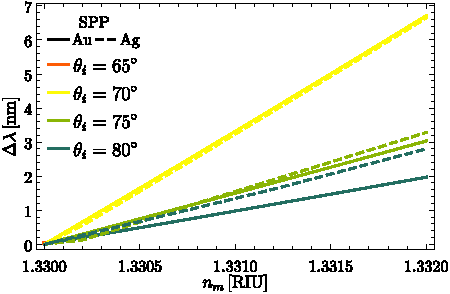
\includegraphics[scale=1]{2-Resultados/figs/11-SPPCSM/4_Sens_h20-SPP.pdf}\end{subfigure}\\
\hspace*{-1.5em}
	\begin{subfigure}{.01\linewidth}\caption{}\label{sfig:FoMCSMp}\vspace{4.5cm}\end{subfigure}
	\begin{subfigure}{.45\linewidth}\hspace*{-.75em}
	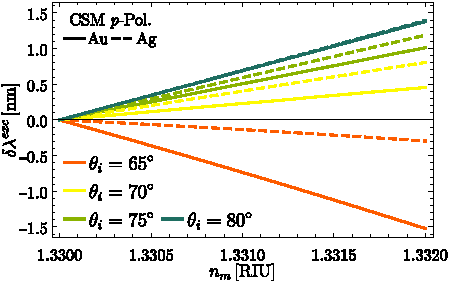
\includegraphics[scale=1]{2-Resultados/figs/11-SPPCSM/5_Sens_h20_CSMP.pdf}\end{subfigure}
	\begin{subfigure}{.01\linewidth}\caption{}\label{sfig:FoMCSMs}\vspace{4.5cm}\end{subfigure}\hspace*{-.75em}
	\begin{subfigure}{.45\linewidth}\centering
	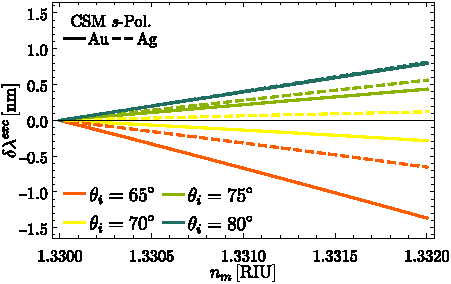
\includegraphics[scale=1]{2-Resultados/figs/11-SPPCSM/6_Sens_h20_CSMS.pdf}\end{subfigure}\vspace*{-.5em}
	\caption{Gráficas del corrimiento $\delta\lambda^{exc}$ de la longitud de onda excitación  en función del índice de refracción de maatriz, en un intervalo entre $1.33$ RIU y $1.332$ RIU, del \textbf{a)} SPP excitado en una película de oro (líneas continuas) y de plata (líneas discontinuas) de $50$ nm de grosor cada una, y  \textbf{b)} del supuesto modo  plasmónico colectivo predicho por el CSM considerando polarización \emph{p} y \textbf{c)}  polarización \emph{s}, excitados en una monocapa de NPs de oro de radio $a=30$ nm y fracción de llenado $\Theta=0.125$ (líneas continuas) y una de NPs de plata con $a=40$ nm y $\Theta=0.1$ (líneas discontinuas).}\label{fig:FoMSPPCSM}
	\end{figure}	

La sensibilidad del SPP [Fig. \ref{sfig:FoMSPP}] sólo se reporta para $\theta_i=70^\circ,\, 75^\circ$ y $80^\circ$ dado que para $65^\circ$ el SPP no se excita en el espectro visible. Sin embargo, la sensibilidad del SPP, tanto para oro como para plata, es mayor al considerar ángulos de incidencia  menores, como se observa al comparar el corrimiento al rojo para $\theta_i=70^\circ$ (líneas amarillas) y  para $\theta_i=80^\circ$ (líneas turquesas).  Considerando un ángulo de incidencia de $70^\circ$ la sensibilidad del SPP para ambos materiales es aproximadamente igual mas para $\theta_i=75^\circ$ y $80^\circ$ el SPP de la película de plata es más sensible que la del oro. El corrimiento al rojo del SPP (para oro y para plata) más amplio con los parámetros escogidos para la Fig. \ref{sfig:FoMSPP} es de $7$ nm cuando el índice de refracción de la matriz  aumenta de $1.33$ RIU a $1.332$ al considerar $\theta_i=70^\circ$.

A diferencia del SPP, el supuesto modo  plasmónico colectivo predicho por el CSM sí puede excitarse en el espectro visible para ángulos cercanos al ángulo crítico y, es en estos valores cuando el supuesto modo  plasmónico colectivo es más sensible, presentando un corrimiento al azul en lugar de un corrimiento al rojo, como se observa en las Figs. \ref{sfig:FoMCSMp} y de la Fig. \ref{sfig:FoMCSMs}, para polarización \emph{p} y \emph{s}, respectivamente. El corrimiento al azul se observa para polarización \emph{p} en $\theta_i=65^\circ$ y, para este ángulo de incidencia, la monocapa de NPs de oro (línas continuas) es más sensible que para la monocapa de NPs de plata (líneas discontinuas). Para ambos materiales considerados considerando $\theta_i\geq 75^\circ$ (lineas verdes) el supuesto modo  plasmónico colectivo  para las dos polarizaciones,  se corre al rojo; la sensibilidad de la monocapa de NPs de plata es mayor en comparación a la de NPs de oro (ver líneas continuas y discontinuas del mismo color). La sensibilidad del supuesto modo  plasmónico colectivo se maximiza en dos casos: para ángulos de incidencia lo más cercanos al crítico (como también ocurre para el SPP)  y para ángulos de incidencia alrededor de $80^\circ$.   En las Figs. \ref{sfig:FoMCSMp} y \ref{sfig:FoMCSMs} se observa que el mayor corrimiento al rojo para el supuesto modo  plasmónico colectivo predicho por el CSM en polarización \emph{p} y \emph{s} es $\delta\lambda^{exc} \approx -1.5$ nm considerando $\theta_i=65^\circ$.

Se calcula la $\textit{FoM}_B$ para el SPP y el supuesto modo  plasmónico colectivo con base en las Figs. \ref{fig:SPPCSM} y \ref{fig:FoMSPPCSM}; los resultados se presentan en la tabla \ref{tab:FoM}. La FoM de bulto del SPP para el oro es menor a la de la plata para todos los ángulos de incidencia pero son del mismo orden de magnitud. La $\textit{FoM}_B$ de la plata es mayor a la del oro debido a una mayor sensibilidad y a un ancho de resonancia menor. En contrate, la FoM de bulto de la monocapa de NPs, tanto para oro como para plata, es un orden de magnitud menor a la del SPP. La diferencia entre las FoM del SPP y del supuesto modo plasmónico colectivo no se debe  la sensibilidad sino al ancho de la resonancia, el cual aumenta para ángulos de incidencia cercanos al crítico para el  modo plasmónico colectivo.

\begin{table}[h!]
\centering
\caption{Resultados de la figura de mérito $\textit{FoM}_B$ del SPP y del supuesto modo  plasmónico colectivo predicho por el CSM, a ambas polarizaciones, para los ángulos de incidencia $\theta_i = 65^\circ,\,70^\circ,\, 75^\circ$ y $80^\circ$. Para el SPP de consideró una película delgada de oro, y una de plata, de $50$ nm de grosor y para el supuesto modo  plasmónico colectivo, una monocapa de NPs de oro de radio $a=30$ nm y una fracción de cubierta $\Theta=0.125$, y una monocapa de NPs de plata con $a=40$ nm y $\Theta=0.1$.}\vspace*{-.7em}
\label{tab:FoM}\small
%\resizebox{\textwidth}{!}{%
\begin{tabular}{c||c||ccc}
Au & SPP  & CSM \emph{p}-Pol. 	& CSM \emph{s}-Pol. \\ 
$\theta_i$ &  $\textit{FoM}_B$ [$\pm 0.6$ RIU$^{-1}$]	  &  $\textit{FoM}_B$ [$\pm 0.07$ RIU$^{-1}$]		&  $\textit{FoM}_B$  [$\pm 0.04$ RIU$^{-1}$]\\ \hline
$65^\circ$ & --			  &	$-2.64$ & $-0.59$\\
$70^\circ$ & $67.5$ &	$0.93$ & $1.88$\\
$75^\circ$ & $48.5$ &	$2.47$ & $3.19$\\
$80^\circ$ & $69.7$ &	$4.03$ & $4.37$\\
\hline \hline
Ag & SPP  & CSM \emph{p}-Pol. 	& CSM \emph{s}-Pol. \\ 
$\theta_i$ &  $\textit{FoM}_B$ [$\pm 0.2$ RIU$^{-1}$]	  &  $\textit{FoM}_B$ [$\pm 1.1$ RIU$^{-1}$]		&  $\textit{FoM}_B$  [$\pm 0.05$ RIU$^{-1}$]\\ \hline
$65^\circ$ & -- 			  &	$-3.66$ & $-2.08$\\
$70^\circ$ & $90.2$ &	$-0.82$ & $0.42$\\
$75^\circ$ & $64.7$ &	$1.47$  & $2.28$\\
$80^\circ$ & $66.7$ &	$3.31$  & $3.09$
\end{tabular}
\end{table}


Los resultados obtenidos para la sensibilidad y la figura de mérito de bulto del SPP son consistentes con la literatura encontrada \cite{estevez2014trends,danilov2018ultra,svedendahl2009refractometric}. Asimimso, se estima que la figura de mérito de biosensores basados en LSPRs por ejemplo para la NDs-LSPR, es del orden de la unidad \cite{svedendahl2009refractometric}, al igual que la FoM de bulto calculada para el supuesto modo  plasmónico colectivo. A partir de estos resultados se estima que los sensores basados en SPP sean una mejor opción para el biosensado en comparación con sensores nanoestructurados. Sin embargo, la aplicación de sensores basados en NPs  se ha enfocado en el bioreconocimiento en tiempo real \cite{estevez2014trends,svedendahl2009refractometric}, es decir, en la detección de pocas partículas alrededor de la nanoestructura empleada que cambien el índice de refracción de la matriz localmente alrededor de las NPs y no el índice de refacción de toda la matriz. La comparación del SPP  con el supuesto modo colectivo mediante la $\textit{FoM}_B$ no considera los fenómenos en locales alrededor de las nanoestrucutras.